\chapter{Pure functional event-driven ABS}
\label{ch:eventdriven}
In this chapter we build on the previous discussion of update strategies in Chapter \ref{ch:impl_abs} and the implementation techniques presented in the time-driven approach of Chapter \ref{ch:timedriven} to develop concepts for event-driven ABS in a pure functional way. 

\medskip

In event-driven ABS \cite{meyer_event-driven_2014}, the simulation is advanced through events. Agents and the environment schedule events into the future and react to incoming events scheduled by themselves, other agents, the environment or the simulation kernel. Time is discrete in this approach and it advances step-wise from event to event, where each event has an associated receiver and $\Delta t$, indicating the delay to the current virtual simulation time when the event should be scheduled. This implies that time could stay constant, for example when an event is scheduled with $\Delta t = 0$ the virtual simulation time does not advance. Further, agents can schedule events to themselves, emulating a recurring behaviour, which in turn emulates proactive behaviour. Because agents can adopt and change their state and behaviour when processing an event, this means that even if time does not advance, agents can change. This non-signal behaviour is the fundamental difference to the time-driven approach in Chapter \ref{ch:timedriven}. Further, this mechanism is used to implement synchronous agent interactions purely functional as discussed in the respective sections below.

The event-driven approach makes the simulation kernel technically closely related to a Discrete Event Simulation \cite{zeigler_theory_2000}. Due to the necessity of imposing a correct ordering of events in this type of ABS, it needs to be stepped event by event, with the \textit{sequential} update strategy, as introduced in Chapter \ref{sec:seq_strategy}. It is important to emphasise that only the semantics of the sequential update strategy allow the kind of features  presented in the following sections, as the agents act one after the other, seeing the effects of previous agents in the same time step. This would not make sense in the parallel update strategy as used in time-driven ABS, where agents act conceptually at the same time. This means that event-driven ABS is inherently sequential due to its fundamental reliance on effects as will become clearer in the sections below. There exists also Parallel Discrete Event Simulation \cite{fujimoto_parallel_1990}, which processes events in parallel and deals with inconsistencies by reverting to consistent states. We hypothesise that a pure functional approach could be beneficial in such an approach due to persistent data structures and explicit handling of side effects but we leave this for further research.

\medskip

We start the chapter by introducing the concepts of agent identity and event scheduling using an event-driven agent-based SIR model, inspired by \cite{macal_agent-based_2010}. We then use the highly complex Sugarscape model as introduced in Chapter \ref{sec:sugarscape}, to develop more advanced features of ABS in a pure functional context: dynamic creation and removal of agents during simulation, adding a shared mutable environment, local mutable agent state and synchronous agent interactions. 
%Note that the Sugarscape model is not a real event-driven model like the event-driven SIR one is as in it the agents do schedule events but they don't do this into the future - events in Sugarscape don't have associated time-stamps.

\section{Basics of event-driven ABS}
\label{sec:eventdriven_basics}

In this section we derive the basics of event-driven ABS using the SIR model, as introduced in Chapter \ref{sec:sir_model}, with an event-driven approach inspired by \cite{macal_agent-based_2010}. Although it is a fundamentally different approach to ABS than the time-driven implementation in Chapter \ref{sec:timedriven_firststep} both solutions are quantitatively equal as they produce the same class of dynamics. Qualitatively they fundamentally differ though in terms of expressivity and performance as we will see in the discussion.

The basics of event-driven ABS are the concept of agent identity, events and event-scheduling. We introduce them step-by-step using various Monads and then generalise to a \textit{tagless final} approach, which has various benefits as pointed out in the respective section. 

\subsection{An event-driven SIR}
Before we can derive implementation concepts, we first need to discuss how an event-driven SIR model works, as inspired by \cite{macal_agent-based_2010}. Fundamentally, what is required is to transform all time-dependent behaviour and agent interactions into the scheduling and receiving of events. For the SIR this should be trivial and straightforward, taking inspiration from the time-driven implementation, where we simply translate the occurrences of events generated by \textit{occasionally} into scheduling of events. For agent interactions we also use events, making this more explicit than in the time-driven approach. As already pointed out, assuming that events have a receiver and a scheduling time given as $\Delta t$ relative to the current simulation time, we end up with three event-types:

\begin{enumerate}
	\item \textbf{MakeContact} - is used to let susceptible agents pro-actively make contact with $\beta$ (contact rate) other agents per 1 time-unit.
	\item \textbf{Contact$_{Sender, \ SIRState}$} - is used to make contact between agents where, agents reveal their state by sending or replying their current state.
	\item \textbf{Recover} - is used to let infected agents recover pro-actively after the given $\delta$ (illness duration). 
\end{enumerate}

Now we can give a concise definition of all three agent behaviours:

\paragraph{Susceptible Agent}
\begin{itemize}
	\item A susceptible agent initially schedules a \textit{MakeContact} event with $\Delta t = 1$ to itself.
	\item When receiving \textit{MakeContact}, the agent sends a \textit{Contact} event to $\beta$ (contact rate) random other agents with $\Delta t = 0$ and \textit{SIRState} of \textit{Susceptible}, resulting in these events to be scheduled immediately. Further, the agent schedules \textit{MakeContact} with $\Delta t = 1$ to itself, to keep the pro-active process of making contact with other agents active.
	\item When the agent receives a \textit{Contact} event, it checks if it is from an infected agent (\textit{SIRState} is \textit{Infected}). If the event is not from an infected agent, it ignores it, otherwise it becomes infected with a given probability.
\end{itemize}

\paragraph{Infected Agent}
\begin{itemize}
	\item An infected agent initially schedules a \textit{Recover} event to itself, with an exponentially distributed random $\Delta t$ of $\delta$ (illness duration).
	\item When the agent receives a \textit{Contact} event, it checks if it is from a susceptible agent (\textit{SIRState} is \textit{Susceptible}). If the event is not from a susceptible agent, it ignores it, otherwise it simply replies to this susceptible agent with a \textit{Contact} event with $\Delta t = 0$ and and \textit{SIRState} of \textit{Infected}.
\end{itemize}

\paragraph{Recovered Agent}
The recovered agent does not change any more, reacts to no incoming events and schedules no events - it stays constantly \textit{Recovered} forever.

\medskip

It is easy to see that this behaviour emulates the time-driven one and indeed in Figure \ref{fig:sir_eventdriven_dynamics} it is also visually clear that it produces similar dynamics. A striking difference are the small spikes and steps in the dynamics, which stem from the fact that time advances discretely and not continuous as in the time-driven implementation. In Chapter \ref{ch:sir_invariants}, we use property-based testing to show that both implementations indeed produce similar distributions in their dynamics, thus putting the claim that both implementations are quantitatively equal on a much more robust ground.

\begin{figure}
	\centering
	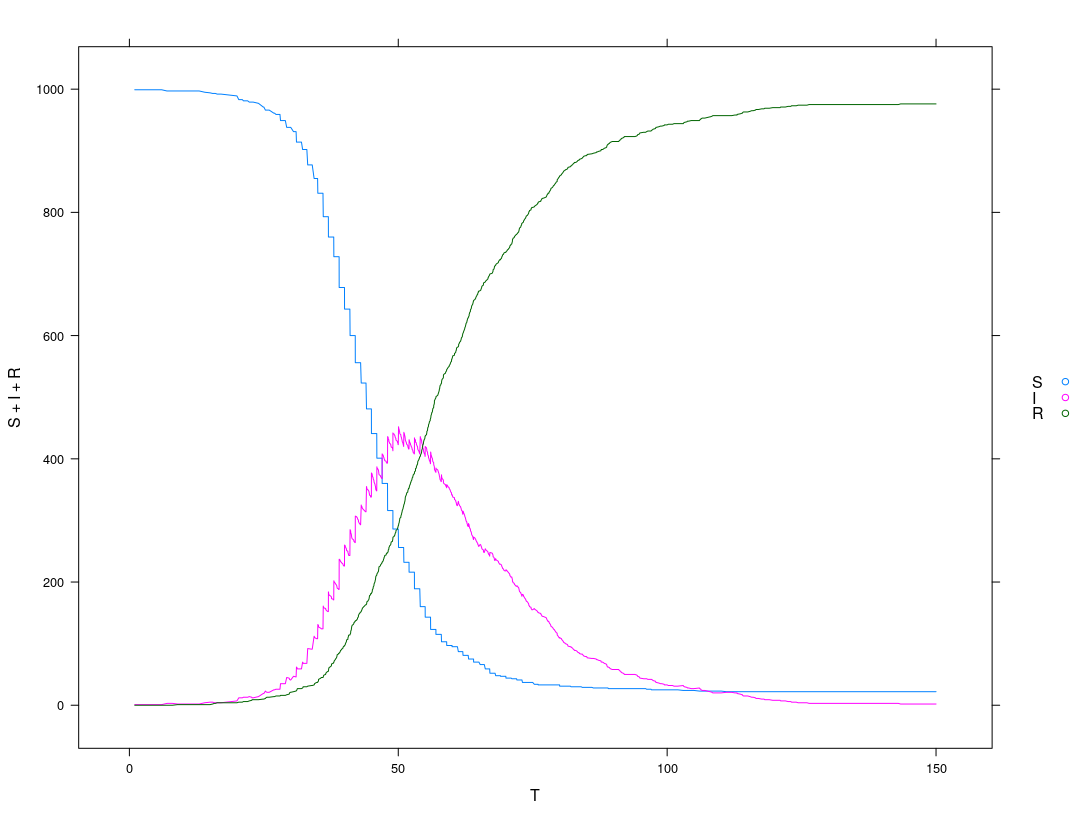
\includegraphics[width=0.7\textwidth, angle=0]{./fig/eventdriven/sir_eventdriven.png}
	\caption{Dynamics of the event-driven SIR model. Population Size $N$ = 1,000, contact rate $\beta = \frac{1}{5}$, infection probability $\gamma = 0.05$, illness duration $\delta = 15$ with initially 1 infected agent. Simulation run for 150 time-steps.}
	\label{fig:sir_eventdriven_dynamics}
\end{figure}

\subsection{Events, Agent Identity and Scheduling}
We can now start to discuss the concepts from an implementation perspective. First, we need to make the concept of an event explicit: they are of a given type, have a receiver and a time-stamp in \textit{absolute} simulation time when they shall be scheduled. We keep the event-type polymorphic and represent the receiver by an \textit{AgentId} which is a simple \textit{Int}. For efficient scheduling, the events are kept in a priority-queue \footnote{We are using the \textit{Data.PQueue.Min} implementation from the \textit{pqueue} package.}, sorted ascending by the time-stamp. Thus we define the following:

\begin{HaskellCode}
type Time        = Double
type AgentId     = Int
data QueueItem e = QueueItem e AgentId Time

-- the event priority-queue
type EventQueue e = PQ.MinQueue (QueueItem e)

-- implement Ord for QueueItem for acended sorting
instance Ord (QueueItem e) where
  compare (QueueItem _ _ t1) (QueueItem _ _ t2) = compare t1 t2
\end{HaskellCode}

Next, we define a polymorphic type for the agent. In event-driven ABS, due to the fact that agents are not signals any more, we abandon time-aware signal functions of BearRiver from the previous chapter and focus solely on Monadic Stream Functions (MSF). In event-driven ABS agents receive events, thus as input to an \textit{MSF} the polymorphic event type \textit{e} is used. As output, the polymorphic output type \textit{o} is used, which will be instantiated to a specific monomorphic type in the SIR model below. The question is now what Monad shall be used. For scheduling purposes (and because models might require it), agents should be able to \textit{read} the current simulation time: this is accomplished through a \textit{ReaderT Time}. Further, agents should be able to \textit{read} the identities of the other agents available in the simulation so they can schedule events to them when necessary: this is accomplished through a \textit{ReaderT [AgentId]}. Most importantly, agents have to be able to schedule events, meaning they have to be able to \textit{write} the events into some sink where they are accumulated for scheduling: this is accomplished through a \textit{WriterT [QueueItem e]}. Finally, the transformer stack needs to be extendible by other Monads, specified in concrete models like the SIR below, so we add another polymorphic type \textit{m}, indicating the closing Monad (stack).

\begin{HaskellCode}
type ABSMonad m e   = ReaderT Time (WriterT [QueueItem e] (ReaderT [AgentId] m))
type AgentMSF m e o = MSF (ABSMonad m e) e o
\end{HaskellCode}

Note that BearRivers \textit{SF} has also a \textit{ReaderT Double} as the innermost Monad but we deliberately avoided its use because the intended semantics of an \textit{SF} are different: the value in the \textit{ReaderT} of the \textit{SF} represents the sampling time-delta and not the absolute time, as in the event-driven case.

We can already implement a few polymorphic functions, operating on the given Monad stack. First, we implement a function \textit{allAgentIds} which simply returns the \textit{AgentId} of all agents, the contents of the \textit{ReaderT [AgentId]}. Second, we implement a function \textit{scheduleEvent} which allows to schedule a given event to a given receiver into the future given a specific time-delay, relative to the current simulation time.
 
\begin{HaskellCode}
allAgentIds :: Monad m => (ABSMonad m e) [AgentId]
allAgentIds = lift (lift ask)

scheduleEvent :: Monad m
              => e        -- ^ event
              -> AgentId  -- ^ receiver
              -> Double   -- ^ time-delay
              -> (ABSMonad m e) ()
scheduleEvent e aid dt = do
  -- get current simulation time
  t <- ask
  -- construct queue item
  let q = QueueItem e aid (t + dt)
  -- write/append (tell) to the WriterT (QueueItem e)
  lift (tell [q])
\end{HaskellCode}

Processing events can also be implemented generically and is straight forward, thus we only discuss the subtleties. For efficient lookup of event receivers all agents are organised into an \textit{IntMap}, which also holds the current output of the agent, to allow sampling of the domain-state. In general, the domain-state is highly model specific, thus a generic implementation needs to offer some mechanism to update the domain-state after an event, a process we named domain-state sampling. Our approach is to call a function which receives the agent map and returns a new domain-state for the current event/time-step. These domain-states are appended to an infinite list which forms the output of the simulation.

The events are then processed in the order provided by the queue and each event is executed with the given receiver. Running a receiver is simply achieved using the agent map, where a reviver is looked up and its \textit{MSF} is evaluated with the given event as input and the resulting monadic actions executed with the given information.
 
\subsection{Parametrising for SIR}
With the generic concepts now established, we show how to parametrise them to the concrete SIR model. First, we define the already well known states the agents can be in and the three different event types, as already introduced above.

\begin{HaskellCode}
data SIRState = Susceptible | Infected | Recovered
data SIREvent = MakeContact | Contact AgentId SIRState | Recover 
\end{HaskellCode}

Next, we parametrise the \textit{ABSMonad} to the SIR model: because behaviour is stochastic, we need to make use of the \textit{Rand} Monad, which also closes the Monad stack of \textit{ABSMonad}. Further, the event type is obviously parametrised to \textit{SIREvent}.

\begin{HaskellCode}
type SIRMonad g = ABSMonad (Rand g) SIREvent
\end{HaskellCode}

Now we define a \textit{SIRAgent} which can be understood as a constructing function, run once upon construction of the agent. This constructing functions runs in the \textit{SIRMonad}, thus agents can already make full use of the functionality, so they can schedule initial events, depending on their initial state. This is important for the susceptible and infected agent, which both need to schedule initial events for pro-active behaviour. The constructing functions also takes the \textit{AgentId} of the agent, thus making it available to the agent at construction time. It returns the initial agent-behaviour as \textit{AgentMSF}.

\begin{HaskellCode}
type SIRAgent g 
       = AgentId -> (SIRMonad g) (AgentMSF (SIRMonad g) SIREvent SIRState)
\end{HaskellCode}

The implementation of the constructing function of type \textit{SIRAgent} is straight forward and follows the specification given above. It makes use of the functions \textit{scheduleMakeContact} and \textit{scheduleRecovery} which are implemented using the generic \textit{scheduleEvent} from above.

\begin{HaskellCode}
sirAgent :: RandomGen g 
         => Int         -- ^ contact rate (beta)
         -> Double      -- ^ infectivity (gamma)
         -> Double      -- ^ illness duration (delta)
         -> SIRState    -- ^ initial state of the agent
         -> SIRAgent g
sirAgent beta gamma delta Susceptible aid = do
  -- on start, schedule MakeContact to itself
  scheduleMakeContact aid 1
  -- return susceptible behaviour
  return (susceptibleAgent aid beta gamma delta)
sirAgent _ _ delta Infected aid = do
  -- on start, schedule Recover to itself
  scheduleRecovery aid delta
  -- return infected behaviour
  return (infectedAgent aid)
sirAgent _ _ _ Recovered _ = 
  -- simply return recovered behaviour
  return recoveredAgent

scheduleMakeContact :: RandomGen g => AgentId -> Double -> (SIRMonadT g) ()
scheduleMakeContact aid = scheduleEvent MakeContact aid

scheduleRecovery :: RandomGen g => AgentId -> Double -> (SIRMonadT g) ()
scheduleRecovery aid delta = do
  dt <- (lift . lift . lift) (randomExpM (1 / delta))
  scheduleEvent Recover aid dt

-- returns random value following exponential distribution with given lambda
randomExpM :: MonadRandom m => Double -> m Double
\end{HaskellCode}

Now we are finally ready to implement the actual behaviour of an agent, where we discuss the full implementation of the susceptible agent behaviour. The basic structure should be already familiar from the time-driven approach, using \textit{switch} to dynamically change the behaviour to \textit{infectedAgent} in case of an infection. The behaviour is then a simple event handler, pattern matching on the incoming events:

\begin{HaskellCode}
susceptibleAgent :: RandomGen g 
                 => AgentId        -- ^ agents id
                 -> Int            -- ^ contact rate (beta)
                 -> Double         -- ^ infectivity (gamma)
                 -> Double         -- ^ illness duration (delta)
                 -> SIRAgentMSF g
susceptibleAgent aid beta gamma delta = 
    switch susceptibleAgentInfected (const (infectedAgent aid))
  where
    susceptibleAgentInfected :: RandomGen g 
                             => MSF (SIRMonadT g) SIREvent (SIRState, Maybe ()) 
    susceptibleAgentInfected = proc e -> do
      -- handle incoming event in monadic action
      ret <- arrM handleEvent -< e
      case ret of
        Nothing -> returnA -< (Susceptible, ret)
        _       -> returnA -< (Infected, ret)
\end{HaskellCode}

We strictly follow the specification as above. In case the agent receives \textit{Contact} from an infected agent it might become infected with a given probability. If it becomes infected, it schedules the recovery as it will make the transition to an infected agent.

\begin{HaskellCode}
-- received Contact from an Infected agent
handleEvent :: RandomGen g => SIREvent -> (SIRMonadT g) (Maybe ())
handleEvent (Contact _ Infected) = do
  -- become infected with gamma probability
  r <- (lift . lift . lift) (randomBoolM gamma)
  if r
    -- got infected 
    then do
      -- schedule Recovery to self, because switching to infected
      scheduleRecovery aid delta
      return (Just ())
    -- no infection
    else return Nothing

-- returns True with given probability
randomBoolM :: MonadRandom m => Double -> m Bool
\end{HaskellCode}

In case the agent receivers \textit{MakeContact} from itself, it will send \textit{Contact} with \textit{Susceptible} to $\beta$ (contact rate) other agents without delay and \textit{MakeContact} to itself with a delay of 1 time unit.

\begin{HaskellCode}
-- received MakeContact (from itself)
handleEvent MakeContact = do
  ais <- allAgentIds
  -- get beta random agents
  receivers <- (lift . lift . lift) (forM [1..beta] (const (randomElemM ais)))
  -- make contact with random agents
  mapM_ makeContactWith receivers
  -- re-schedule MakeContact to self
  scheduleMakeContact aid 1
  return Nothing
  
makeContactWith :: AgentId -> (SIRMonadT g) ()
makeContactWith receiver = 
  -- schedule Contact event immediately
  scheduleEvent (Contact aid Susceptible) receiver 0

-- picks an element randomly from the (non empty) list
randomElemM :: MonadRandom m => [e] -> m e
\end{HaskellCode}

The infected and recovered behaviours are conceptually equivalent and thus left as a trivial exercise to the reader. 

\subsection{Tagless Final}
At this point, the basics of event-driven ABS should be clear: how events are represented and processed using an event queue, how agents are represented with an \textit{MSF} and the idea behind the underlying polymorphic Monad transformer stack. Further, by parametrising the polymorphic concepts to the SIR model, we showed how to instantiate the generic concepts into a concrete model to arrive at a robust, maintainable and solid solution which is very likely to be correct up to the initial informal specification.

\medskip

In this section we briefly want to show how the so-called \textit{tagless final} approach \cite{kiselyov_typed_2012} can be used to arrive at a cleaner and more extensible interface of our implementation, which is also open to different \textit{interpretations}. The idea behind \textit{tagless final} is simple: specify the interface of operations in a typeclass and then write one or multiple interpreters for it, which simply means writing an instance implementation for the given typeclass. We start by defining the typeclass \textit{MonadAgent} with all the necessary methods, making up the effectful API of our agents. Note that we need to enable two language extensions: \textit{MultiParamTypeClasses} because we want to have more than a single type parameter in the typeclass - besides the Monad \textit{m}, we also want to parametrise over the event type \textit{e}; \textit{FunctionalDependencies} because the event type \textit{e} is determined by the Monad type \textit{m}.

\begin{HaskellCode}
{-# LANGUAGE MultiParamTypeClasses  #-}
{-# LANGUAGE FunctionalDependencies #-}

class Monad m => MonadAgent e m | m -> e where
  randomBool  :: Double -> m Bool
  randomExp   :: Double -> m Double
  randomElem  :: [a] -> m a
  getAgentIds :: m [AgentId]
  getTime     :: m Time
  getMyId     :: m AgentId
  schedEvent  :: e -> AgentId -> Double -> m ()
\end{HaskellCode}

The methods are self explaining. This typeclass is now used to replace the Monad stack by an overloaded type definition in the respective functions. Thus, the implementation of the agent constructing function and the agent behaviours are the same, with only the types changing slightly, lifts becoming obsolete and calls to function replaced by calls to methods of the typeclass. We don't give the full implementation again but only the type of the agent construction function as example, the types of the agent behaviours follow a similar pattern: 

\begin{HaskellCode}
sirAgent :: MonadAgent SIREvent m  -- CHANGED: overloaded with typeclass
         => Int         -- ^ contact rate (beta)
         -> Double      -- ^ infectivity (gamma)
         -> Double      -- ^ illness duration (delta)
         -> SIRState    -- ^ initial state of the agent
         -> m (MSF m SIREvent SIRState) -- CHANGED: no Monad stack
\end{HaskellCode}

Note that we added a \textit{getMyId} method, which shall return the \textit{AgentId} of the agent itself, avoiding the need for the agent of keeping the agent id around and also making it possible to implement more robust self-scheduling functions. For example, the \textit{scheduleRecovery} function is implemented in the \textit{tagless final} approach in the following way:

\begin{HaskellCode}
scheduleRecovery :: MonadAgent SIREvent m => Double -> m ()
scheduleRecovery delta = do
  -- draw random value from exponential distribution
  dt <- randomExp (1 / delta)
  -- get id of agent, no more need to pass it explicitly
  ai <- getMyId
  -- schedule Recover to itself
  schedEvent Recover ai dt
\end{HaskellCode}

What we are missing is a \textit{pure} interpreter for the agent implementation and the \textit{MonadAgent} typeclass. We start by defining a \textit{newtype}, which basically is a conceptually similar Monad stack as in the original implementation without the \textit{tagless final} approach. We let Haskell automatically derive monadic typeclasses, Functor, Applicative and Monad instances which saves a lot of boiler plate code, for which the \textit{GeneralizedNewtypeDeriving} language extension is required. Instead of the \textit{Rand} Monad, a \textit{StateT SimState} is used, which carries the random-number generator and other data  for synchronous agent interactions as will be discussed in the respective sections.

\begin{HaskellCode}
{-# LANGUAGE GeneralizedNewtypeDeriving #-}

newtype SIRAgentPure a = SIRAgentPure 
  { unSirAgentPure :: ReaderT (Time, AgentId, [AgentId]) -- combined into one
                        (WriterT [QueueItem SIREvent]
                          (State SimState)) a}
  deriving (Functor, Applicative, Monad, 
            MonadReader (Time, AgentId, [AgentId]),
            MonadWriter [QueueItem SIREvent],  
            MonadState SimState)
\end{HaskellCode}

Having this \textit{newtype} we can now write a \textit{pure} interpreter for the \textit{MonadAgent}. The implementations are straight forward and should be self explanatory. To run \textit{Rand} Monad actions, the function \textit{runRandWithSimState} is used, which extracts the random-number generator from \textit{SimState}, runs the action and puts the changed random-number generator back into the \textit{SimState}.

\begin{HaskellCode}   
{-# LANGUAGE FlexibleContexts           #-}
{-# LANGUAGE MultiParamTypeClasses      #-}
      
instance MonadAgent SIREvent SIRAgentPure where
  randomBool = runRandWithSimState . randomBoolM
  randomElem = runRandWithSimState . randomElemM
  randomExp  = runRandWithSimState . randomExpM
  -- schedEvent :: SIREvent -> AgentId -> Double -> m ()
  schedEvent e receiver dt = do
    t <- getTime 
    tell [QueueItem e receiver (t + dt)]
  -- getAgentIds :: m [AgentId]
  getAgentIds = asks trd
  -- getTime :: m Time
  getTime = asks fst3
  -- getMyId :: m AgentId
  getMyId = asks snd3

fst3 :: (a,b,c) -> a
snd3 :: (a,b,c) -> b
trd :: (a,b,c) -> c
runRandWithSimState :: MonadState SimState m => Rand StdGen a -> m a
\end{HaskellCode}

The main benefit of a \textit{tagless final} approach is that it is a solution to the expression problem \cite{kiselyov_typed_2012}: it is possible to add new interpreters of an embedded language and add new functionality without breaking the existing implementations. Interpretation in our case means that we can use different underlying Monads to run the agents: if we want to guarantee purity, no \textit{IO} Monad shall be used. Otherwise when concurrency with a lock-based approach or a lock-free approach is required \textit{IO} or \textit{STM} can be used in the underlying interpreter. Also, for reproducible unit testing, one can write custom test-interpreters where methods always return a-priori known results, similar to mocking. Adding new functionality is less an issue here but might become highly important when designing a more general ABS library, building on the \textit{tagless final} approach. It would allow the user of such a library to extend existing agents or default behaviour with new, custom-built methods, without breaking the existing ones. We leave that for further research.

\section{Advanced features}
\label{sec:advanced_eventdriven_ABS}

In the previous section we established the basics of event-driven ABS. It is now clear how events are represented, how agent identity is handled, how agents receive and schedule events, how events are scheduled and domain state is sampled. Furthermore, by using the \textit{tagless final} approach, we arrived at an elegant, extensible and robust solution, which separates specification, the agent and its behaviour, from its implementation, a \textit{pure} interpreter. 

In this section we present more advanced concepts of event-driven ABS, necessary in models with much higher complexity than the simple SIR. We developed these concepts using the Sugarscape model as introduced in Chapter \ref{sec:sugarscape}. Consequently we will discuss them from this model's perspective. More specifically, we show how to create and remove agents dynamically during simulation, add a shared mutable environment, model local mutable agent state and finally how synchronous agent interactions can be implemented. Together with the basics of event-driven ABS, with these concepts established it should be possible to implement a wide range of event-driven ABS models. For this we developed a full implementation of the Sugarscape model, in which we explored the concepts presented in this chapter, with the code accessible from the \href{https://github.com/thalerjonathan/haskell-sugarscape}{code repository}~\cite{thaler_sugarscape_repository}.

\section{Case Study II: Sugarscape}
\label{sec:sugarscape_concurrent}
The second case study is the Sugarscape model as introduced in Chapter \ref{sec:sugarscape}. In this case study we look into the potential performance improvement in a model with much more complex agent behaviour and dramatically increased writes on the shared environment.

We implemented the \textit{Carrying Capacity} (p. 30) section of Chapter II of the Sugarscape book \cite{epstein_growing_1996}. In each step agents search (move) to the cell with the most sugar they see within their vision, harvest all of it from the environment and consume sugar because of their metabolism. Sugar regrows in the environment over time. Only one agent can occupy a cell at a time. Agents don't age and cannot die from age. If agents run out of sugar due to their metabolism, they die from starvation and are removed from the simulation. The authors report that the initial number of agents quickly drops and stabilises around a level depending on the model parameters. This is in accordance with our results as we show in Chapter \ref{ch:property} and guarantees that we don't run out of agents. The model parameters are as follows:

\begin{itemize}
	\item Sugar Endowment: each agent has an initial sugar endowment randomly uniform distributed between 5 and 25 units;
	\item Sugar Metabolism: each agent has a sugar metabolism randomly uniform distributed between 1 and 5;
	\item Agent Vision: each agent has a vision randomly uniform distributed between 1 and 6, same for each of the 4 directions (N, W, S, E);
	\item Sugar Growback: sugar grows back by 1.0 unit per step until the maximum capacity of a cell is reached;
	\item Agent Number: initially 500 agents;
	\item Environment Size: 50 x 50 cells with toroid boundaries which wrap around in both x and y dimension.
\end{itemize}

Note that in this implementation (as in the full Chapter II of the book), no direct and no synchronous agent-interactions as we implemented them in Chapter \ref{sec:eventdriven_implementation} are happening. As in the SIR example, all agents interact with each other indirectly through the shared environment. This allows us to regard the implementation as a time-driven, parallel one wherein each step agents act conceptually at the same time.

We compare four different implementations \footnote{The code is freely available at \url{https://github.com/thalerjonathan/phd/tree/master/public/stmabs/code/SugarScape}}:

\begin{enumerate}
	\item Sequential - All agents are run after another (including the environment) and the environment is shared amongst the agents using a \textit{StateT} transformer.
	\item Lock-Based - All agents are run concurrently in the \textit{IO} monad and the environment is shared between the agents, using an \textit{IORef} with the access synchronised through an \textit{MVar} lock.
	\item STM TVar - All agents are run concurrently in the \textit{STM} monad and the environment is shared using a \textit{TVar} between the agents.
	\item STM TArray - All agents are run concurrently in the \textit{STM} monad and the environment is shared using a \textit{TArray} between the agents. 
\end{enumerate}

We follow \cite{lysenko_framework_2008} and measure the average number of steps per second of the simulation over 60 seconds. For each experiment we conducted 8 runs on our machine (see Table \ref{tab:machine_specs}) under no additional work-load and report the average. In the experiments we varied the number of cores when running concurrently - the numbers are always indicated clearly.

%\paragraph{Output} Note that we omit the graphical rendering in the functional approach because it is a serious bottleneck taking up substantial amount of the simulation time. Although visual output is often important in ABS, it is not what we are interested here thus we completely omit it and only output the number of agents in the simulation at each step piped into a file, thus omitting slow output to the console \footnote{Note that we need to produce \textit{some} output because of Haskells laziness - if we wouldn't output anything from the simulation then the expressions would actually never be fully evaluated thus resulting in high number of steps per second but which obviously don't really reflect the true computations done.}.

\paragraph{Ordering} The model specification requires to shuffle agents before every step (Footnote 12 on page 26 \cite{epstein_growing_1996}). In the \textit{Sequential} approach we do this explicitly but in the \textit{Lock-Based} and both \textit{STM} approaches we assume this to happen automatically due to race-conditions in concurrency, thus we arrive at an effectively shuffled processing of agents: we implicitly assume that the order of the agents is \textit{effectively} random in every step. The important difference between the two approaches is that in the \textit{Sequential} approach we have full control over this randomness but in the \textit{STM} not - also this means that repeated runs with the same initial conditions might lead to slightly different results. 
This decision leaves the execution order of the agents ultimately to Haskell's Runtime System and the underlying OS. We are aware that by doing this, we make assumptions that the threads run uniformly distributed (fair) but such assumptions should not be made in concurrent programming. As a result we can expect this fact to produces non-uniform distributions of agent runs but we assumed that for this model this does not has a significance influence - in case of doubt, we could resort to shuffling the agents before running them in every step. We agree that this very problem would deserve in-depth research on its own, where also the influence of non-deterministic ordering on the correctness and results of ABS has to be analysed. This is not the main interest of this section though and we leave it for further research as it is completely beyond the focus of this thesis.

%Note that in the concurrent implementations we have two options for running the environment: either asynchronously as a concurrent agent at the same time with the population agents or synchronously after all agents have run. We must be careful though as running the environment as a concurrent agent can be seen as conceptually wrong because the time when the regrowth of the sugar happens is now completely random. In this case it could happen that sugar regrows in the very first transaction or in the very last, different in each step, which can be seen as a violation of the model specifications. Thus we do not run the environment concurrently with the agents but synchronously after all agents have run.

\subsection{Constant Agent Size}
In a first approach we compare the performance of all implementations on varying numbers of cores. The results are reported in Table \ref{tab:varying_cores} and plotted in Figure \ref{fig:varying_cores}. 

\begin{table}
	\centering
	\begin{tabular}{cc|c|c}
		\multicolumn{1}{ c||  }{\multirow{2}{*}{} } &
		\multicolumn{1}{ |c| }{Cores} & Steps & Retries      \\ \hline \hline 
		
		\multicolumn{1}{ c||  }{\multirow{1}{*}{Sequential} } &
		\multicolumn{1}{ |c| }{1} & 39.4 & N/A     \\ \hline \hline 
		
		\multicolumn{1}{ c||  }{\multirow{4}{*}{Lock-Based} } &
		\multicolumn{1}{ |c| }{1} & 43.0 & N/A       \\ \cline{2-4}
		\multicolumn{1}{ c||  }{}                       &
		\multicolumn{1}{ |c| }{2} & 51.8 & N/A   \\ \cline{2-4}
		\multicolumn{1}{ c||  }{}                       &
		\multicolumn{1}{ |c| }{3} & 57.4 & N/A   \\ \cline{2-4}
		\multicolumn{1}{ c||  }{}                       &
		\multicolumn{1}{ |c| }{4} & 58.1 & N/A   \\ \hline \hline 
		
		\multicolumn{1}{ c||  }{\multirow{4}{*}{STM \textit{TVar}} } &
		\multicolumn{1}{ |c| }{1} & \textbf{47.3} & 0.0       \\ \cline{2-4}
		\multicolumn{1}{ c||  }{}                       &
		\multicolumn{1}{ |c| }{2} & 53.5 & 1.1    \\ \cline{2-4}
		\multicolumn{1}{ c||  }{}                       &
		\multicolumn{1}{ |c| }{3} & 57.1 & 2.2    \\ \cline{2-4}
		\multicolumn{1}{ c||  }{}                       &
		\multicolumn{1}{ |c| }{4} & 53.0 & 3.2   \\ \hline \hline 
		
		\multicolumn{1}{ c||  }{\multirow{4}{*}{STM \textit{TArray}} } &
		\multicolumn{1}{ |c| }{1} & 45.4 & 0.0       \\ \cline{2-4}
		\multicolumn{1}{ c||  }{}                       &
		\multicolumn{1}{ |c| }{2} & \textbf{65.3} & 0.02   \\ \cline{2-4}
		\multicolumn{1}{ c||  }{}                       &
		\multicolumn{1}{ |c| }{3} & \textbf{75.7} & 0.04    \\ \cline{2-4}
		\multicolumn{1}{ c||  }{}                       &
		\multicolumn{1}{ |c| }{4} & \textbf{84.4} & 0.05   \\ \hline \hline 
	\end{tabular}  	
  	
  	\caption{Steps per second and retries on 50x50 grid with 500 initial agents on varying cores.}
	\label{tab:varying_cores}
\end{table}

\begin{figure}
	\centering
	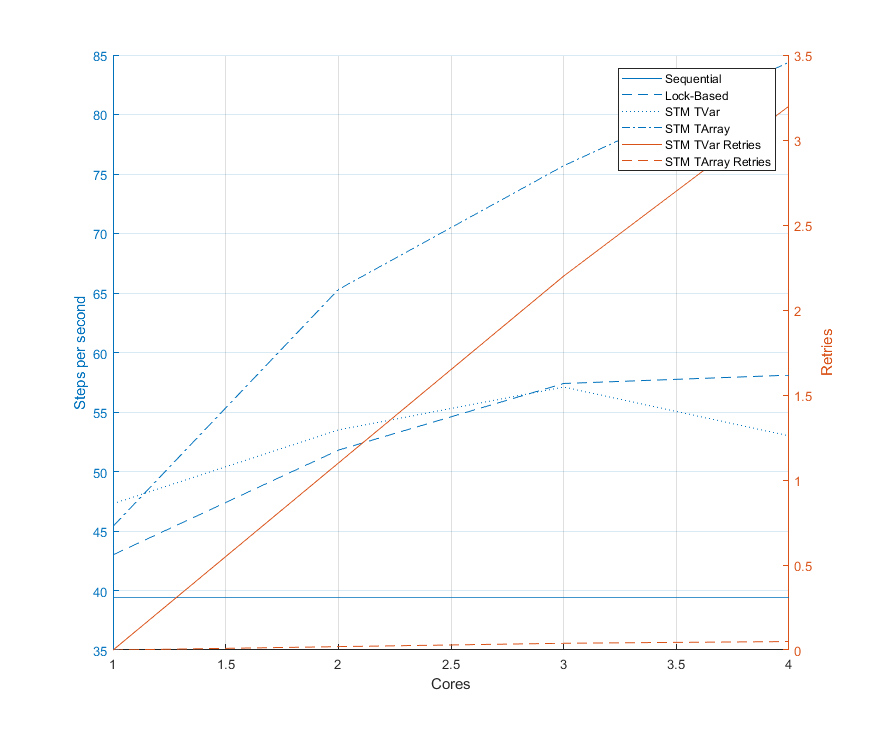
\includegraphics[width=0.7\textwidth, angle=0]{./fig/concurrentabs/sugarscape/varying_cores.png}
	\caption{Steps per second and retries on 50x50 grid and 500 initial agents on varying cores.}
	\label{fig:varying_cores}
\end{figure}

As expected, the \textit{Sequential} implementation is the slowest, followed by the \textit{Lock-Based} and \textit{TVar} approach whereas \textit{TArray} is the best performing one.

We clearly see that using a \textit{TVar} to share the environment is a very inefficient choice in this model: \textit{every} write to a cell leads to a retry independent whether the reading agent reads that changed cell or not, because the data-structure can not distinguish between individual cells. By using a \textit{TArray} we can avoid the situation where a write to a cell in a far distant location of the environment will lead to a retry of an agent which never even touched that cell. Also the \textit{TArray} seems to scale up by 10 steps per second for every core added. It will be interesting to see how far this could go with the Amazon experiment, as we seem not to hit a limit with 4 cores yet.

The inefficiency of \textit{TVar} is also reflected in the nearly similar performance of the \textit{Lock-Based} implementation which even outperforms it on 4 cores. This is due to very similar approaches because both operate on the whole environment instead of only the cells as \textit{TArray} does. This seems to be a bottleneck in \textit{TVar} reaching the best performance on 3 cores, which then drops on 4 cores due to an increasing retries ratio. The \textit{Lock-Based} approach seems to reduce its returns on increased number of cores hitting a limit at 4 cores as well.

\subsection{Scaling up Agents}
So far we kept the initial number of agents at 500, which due to the model specification, quickly drops and stabilises around 200 due to the carrying capacity of the environment as described in the book \cite{epstein_growing_1996} section \textit{Carrying Capacity} (p. 30).

We now want to measure the performance of our approaches under increased number of agents. For this we slightly change the implementation: always when an agent dies it spawns a new one which is inspired by the ageing and birthing feature of Chapter III in the book \cite{epstein_growing_1996}. This ensures that we keep the number of agents roughly constant (still fluctuates but doesn't drop to low levels) over the whole duration. This ensures a constant load of concurrent agents interacting with each other and demonstrates also the ability to terminate and create concurrent agents (threads) dynamically during the simulation.

Except for the \textit{Sequential} approach we ran all experiments with 4 cores (TVar with 3 as well). We looked into the performance of 500, 1,000, 1,500, 2,000 and 2,500 (maximum possible capacity of the 50x50 environment). The results are reported in Table \ref{tab:state_results_agentsscale_time} and plotted in Figure \ref{fig:state_results_agentsscale_time}.

\begin{table}
	\centering
  	\begin{tabular}{ c || c | c | c | c | c }
        Agents  & Sequential & Lock-Based & TVar (3 cores) & TVar (4 cores) & TArray  \\ \hline \hline 
    	    500     & 14.4       & 20.2		  &	20.1           & 18.5       	& \textbf{71.9}    \\ \hline
   		1,000   & 6.8        & 10.8 	      & 10.4           & 9.5         & \textbf{54.8}    \\ \hline
   		1,500   & 4.7        & 8.1 		  & 7.9            & 7.3			& \textbf{44.1}    \\ \hline
   		2,000   & 4.4        & 7.6 		  & 7.4            & 6.7    		& \textbf{37.0}    \\ \hline 
   		2,500   & 5.3        & 5.4 		  & 9.2            & 8.9			& \textbf{33.3}    \\ \hline \hline
   	\end{tabular}
  	
  	\caption{Steps per second on 50x50 grid with varying number of agents with 4 (and 3) cores except Sequential (1 core).}
	\label{tab:state_results_agentsscale_time}
\end{table}

\begin{figure}
	\centering
	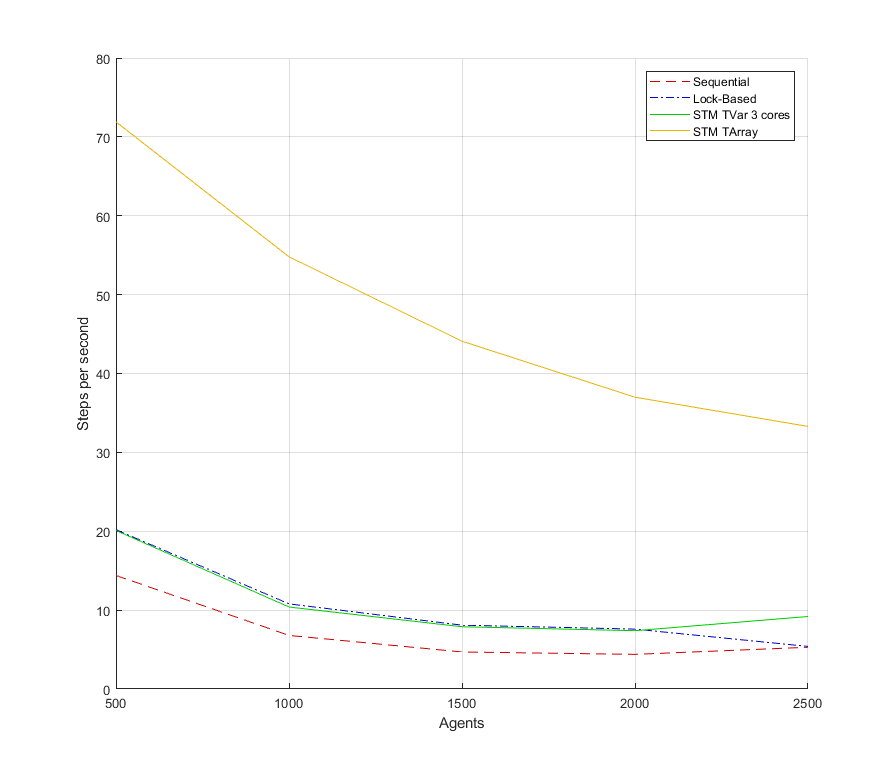
\includegraphics[width=1.0\textwidth, angle=0]{./fig/concurrentabs/sugarscape/varying_agents.png}
	\caption{Steps per second on 50x50 grid and varying number of agents with 4 (and 3) cores except Sequential (1 core).}
	\label{fig:state_results_agentsscale_time}
\end{figure}

As expected, the \textit{TArray} implementation outperforms all others substantially. Also as expected, the \textit{TVar} implementation on 3 cores is faster than on 4 cores as well when scaling up to more agents. The \textit{Lock-Based} approach performs about the same as the \textit{TVar} on 3 cores because of the very similar approaches: both access the \textit{whole} environment. Still the \textit{TVar} approach uses one core less to arrive at the same performance, thus strictly speaking outperforming the \textit{Lock-Based} implementation.

What seems to be very surprising is that in the \textit{Sequential} and \textit{TVar} cases the performance with 2,500 agents is \textit{better} than the one with 2,000 agents. The reason for this is that in the case of 2,500 agents, an agent can't move anywhere because all cells are already occupied. In this case the agent won't rank the cells in order of their pay-off (max sugar) to move to but just stays where it is. We hypothesize that due to Haskells laziness the agents actually never look at the content of the cells in this case but only the number which means that the cells themselves are never evaluated which further increases performance. This leads to the better performance in case of \textit{Sequential} and \textit{TVar} because both exploit laziness.
In the case of the \textit{Lock-Based} approach we still arrive at a lower performance because the limiting factor are the unconditional locks. In the case of the \textit{TArray} approach we also arrive at a lower performance because it seems that STM perform reads on the neighbouring cells which are not subject to lazy evaluation. In Haskell it is notoriously difficult to reason about efficiency (see Chapter \ref{ch:drawbacks} for a short discussion on drawbacks) and this behaviour of improved performance due to Haskells lazyness is no exception. We leave an in-depth investigation for further research as it is beyond the focus of this chapter.

We also measured the average retries both for \textit{TVar} and \textit{TArray} under 2,500 agents where the \textit{TArray} approach shows best scaling performance with 0.01 retries whereas \textit{TVar} averages at 3.28 retries. Again this can be attributed to the better transactional data-structure which reduces retry-ratio substantially to near-zero levels.

\subsection{Going Large-Scale}
To test how far we can scale up the number of cores in both the \textit{Lock-Based} and \textit{TArray} cases, we ran the two experiments (carrying capacity and rebirthing) on Amazon EC2 instances with increasing number of cores starting with 16 and 32 to see if we run into decreasing returns. The results are reported in Table \ref{tab:sug_varying_cores_amazon}.

\begin{table}
	\centering
%  	\begin{tabular}{ c || c | c | c }
%                   & Cores & Carrying Capacity & Rebirthing  \\ \hline \hline 
%    	Lock-Based & 16    & 53.9              & 4.4         \\ \hline
%    	Lock-Based & 32    & 44.2              & 3.6         \\ \hline \hline 
%   		
%   		STM TArray & 16    & \textbf{116.8} (0.23)      & \textbf{39.5} (0.08) \\ \hline
%   		STM TArray & 32    & 109.8 (0.41)      & 31.3 (0.18) \\ \hline \hline 
%   	\end{tabular}
  	
	\begin{tabular}{cc|c|c}
		\multicolumn{1}{ c||  }{\multirow{2}{*}{} } &
		\multicolumn{1}{ |c| }{Cores} & Carrying Capacity    & Rebirthing       \\ \hline \hline 
		
		\multicolumn{1}{ c||  }{\multirow{2}{*}{Lock-Based} } &
		\multicolumn{1}{ |c| }{16} & 53.9              & 4.4       \\ \cline{2-4}
		\multicolumn{1}{ c||  }{}                       &
		\multicolumn{1}{ |c| }{32} & 44.2              & 3.6      \\ \hline \hline 
		
		\multicolumn{1}{ c||  }{\multirow{2}{*}{STM TArray} } &
		\multicolumn{1}{ |c| }{16} & \textbf{116.8} (0.23)      & \textbf{39.5} (0.08)       \\ \cline{2-4}
		\multicolumn{1}{ c||  }{}                       &
		\multicolumn{1}{ |c| }{32} & \textbf{109.8} (0.41)      & \textbf{31.3} (0.18)      \\ \hline \hline 
	\end{tabular}  	
  	
  	\caption{Steps per second on varying cores on Amazon S2 Services.}
	\label{tab:sug_varying_cores_amazon}
\end{table}

As expected, the \textit{Lock-Based} approach doesn't scale up to many cores because each additional core brings more contention to the lock, resulting in even more decreased performance. This is particularly obvious in the rebirthing experiment because of the much larger number of concurrent agents. The \textit{TArray} approach returns better performance on 16 cores but fails to scale further up to 32 where the performance drops below the one with 16 cores. We indicated the retry-ratio in brackets and see that they roughly double from 16 to 32, which is the reason why performance drops as at this point. 

%the INCREASE in time can only happen due to more retries
%Carrying Capacity 16 core ~ 0.23 retry-ratio
%Carrying Capacity 32 core ~ 0.41 retry-ratio
%
%Rebirthing 16 core ~ 0.08 retry-ratio
%Rebirthing 32 core ~ 0.18 retry-ratio

\subsection{Comparison with other approaches}
The paper \cite{lysenko_framework_2008} reports a performance of 17 steps in RePast, 18 steps in MASON (both non-parallel) and 2,000 steps per second on a GPU on a 128x128 grid. Although our \textit{Sequential} implementation, which runs non-parallel as well, outperforms the RePast and MASON implementations of \cite{lysenko_framework_2008}, one must be very well aware that these results were generated in 2008, on current hardware of that time.

%When we run the SugarScape example of RePast with the same model parameters as ours on the same machine (see Table \ref{tab:machine_specs}) we arrive at roughly 450 steps per second - a factor of about 3.8 faster than even our STM \textit{TArray} implementation on 16 cores. This might seem quite shocking, even more so because RePast also performs visual output, rendering the SugarScape in every step. When scaling up the agents to 2,500 the RePast version arrives around roughly 95 steps per second which is still faster by a factor of 3 than our 4 core \textit{TArray} implementation. We attribute this substantial performance difference to the inherent performance difference of functional programming to imperative approaches as already outlined in the previous section. 

The very high performance on the GPU does not concern us here as it follows a very different approach than ours. We focus on speeding up implementations on the CPU as directly as possible without locking overhead. When following a GPU approach one needs to map the model to the GPU which is a delicate and non-trivial matter. With our approach we show that speed up with concurrency is very possible without the low-level locking details or the need to map to GPU. Also some features as bilateral trading between agents, where a pair of agents needs to come to a conclusion over multiple synchronous steps, is difficult to implement on a GPU whereas this is easily possible using STM.

Note that we kept the grid-size constant because we implemented the environment as a single agent which works sequentially on the cells to regrow the sugar. Obviously this doesn't really scale up on parallel hardware and experiments which we haven't included here due to lack of space, show that the performance goes down dramatically when we increase the environment to 128x128 with same number of agents which is the result of Amdahl's law where the environment becomes the limiting factor of the simulation. Depending on the underlying data-structure used for the environment we have two options to solve this problem. In the case of the \textit{Sequential} and \textit{TVar} implementation we build on an indexed array, which we can be updated in parallel using the existing data-parallel support in Haskell. In the case of the \textit{TArray} approach we have no option but to run the update of every cell within its own thread. We leave both for further research as it is out of scope of this paper.

\subsection{Discussion}
This case study showed clearly that besides being substantially faster than the \textit{Sequential} implementation, \textit{STM} is also able to perform considerably better than a \textit{Lock-Based} approach even in the case of a model with much higher complexity in agent behaviour and dramatically increased number of writes to the environment.
Further, this case study demonstrated that the selection of the right transactional data-structure is of fundamental importance when using \textit{STM}. Selecting the right transactional data-structure is very model-specific and can lead to dramatically different performance results.
In this case the \textit{TArray} performed best due to many writes but in the SIR case-study a \textit{TVar} showed good enough results due to the very low number of writes. When not carefully selecting the right transactional data-structure which supports fine-grained concurrency, a lock-based implementation might perform as well or even outperform the STM approach as can be seen when using the \textit{TVar}.
Although the \textit{TArray} is the better transactional data-structure overall, it might come with an overhead, performing worse on low number of cores than a \textit{TVar} approach but has the benefit of quickly scaling up to multiple cores. Depending on the transactional data-structure, scaling up to multiple cores hits a limit at some point. In the case of the \textit{TVar} the best performance is reached with 3 cores. With the \textit{TArray} we reached this limit around 16 cores.

Note that the comparison between the \textit{Lock-Based} approach and the \textit{STM TArray} implementation is a bit unfair due to a very different locking structure. A more suitable comparison would have been to use an indexed Array with a tuple of (MVar, IORef) in each cell to support fine-grained locking on cell-level. This would be a more just comparison to the \textit{STM Array} where fine-grained transactions happen on the cell-level. We hypothesize that \textit{STM} will still outperform the \textit{IO} approach but to a lesser degree - we leave the proof of this for further research.

%Unfortunately, for this model the performance is nowhere comparable to imperative approaches, which we attribute to the inherent performance difference of functional programming to imperative approaches. With the use of advanced language features we might arrive at much improved performance but we leave this for further research as we focus primarily on the comparison between lock-based and STM approaches.

%we can implement everything except synchronous direct agent-interactions atm: if agent-interaction is one-way e.g. paying back a loan then this is no problem. thus the following parts of the Sugarscape are not possible with our current STM approach: mating, trading and lending  because all 3 require direct agent-to-agent interaction over multiple steps. We leave the problem of developing such an algorithm / implementation for further research.

\subsection{Dynamic agent creation and removal}
Some models of ABS in general and Sugarscape in particular require the dynamic creation and removal of agents during simulation. The specific requirements here are that the agents themselves must be able to both remove themselves from the simulation and create new agents with given attributes. To achieve that, in such a simulation the output type of an agent must be richer than the one in the event-driven SIR. First, we define the output of an agent:

\begin{HaskellCode}
data AgentOut m e o = AgentOut
  { aoKill   :: Any              -- True if this agent should be removed 
  , aoCreate :: [AgentDef m e o] -- a list of agents to create
  , aoEvents :: [(AgentId, e)]   -- a list of events (receiver, event)
  }
\end{HaskellCode}

Note that \textit{AgentOut} contains already the list of scheduled events, which makes it clear that scheduling of events in this approach is implemented different than in the event-driven SIR, where the agents Monad stack had a \textit{WriterT} to write events to. The reason for that is that we treat agent-local abstractions different here because of the need to encapsulate local agent state as explained in subsequent sections.

If the agent wants to remove itself from the simulation, it simply sets \textit{aoKill} to True; if it wants to create new agents it adds an agent definition \textit{AgentDef} to the \textit{aoCreate} list. The agent definition \textit{AgentDef} holds the new id of the agent \footnote{Note that an agent-controlled id makes it possible to re-use ids in case an agent dies and in case ids have no other purposes than identifying event receivers in a model}, the MSF of the agent to create and the initial output of the new agent, so it has a representation in the visual or textual output for the current step without the need to run the new agent.

\begin{HaskellCode}
data AgentDef m e o = AgentDef
  { adId      :: AgentId         -- unique agent-id
  , adMSF     :: AgentMSF m e o  -- the agent behaviour function
  , adInitOut :: o               -- the value of the initial output
  }
\end{HaskellCode}

Further, the simulation must provide a \textit{global} mechanism to create new, unique \textit{AgentId} for the newly created agents. The generating of ids for the new agents have to occur within the parent agents themselves because in some models they might need this very id to communicate with their children - an indirection through the kernel would only complicate matters. We thus start with a data definition, holding the next agent id - if an agent creates a new agent it simply reads that value and increments it by 1.

\begin{HaskellCode}
data ABSState = ABSState { absNextId :: AgentId }
\end{HaskellCode}

To make it \textit{globally} available to all agents a \textit{StateT ABSState} Monad transformer is used, which is also the innermost Monad of the Monad stack of Sugarscape \footnote{In the Sugarscape implementation, \textit{ABSState} also holds the current simulation time, which is omitted here for clarity reasons.}.

\begin{HaskellCode}
type AgentMonad m = StateT ABSState m
\end{HaskellCode}

Finally, we can define the polymorphic type of the agent MSF, as it is used in Sugarscape, where it is parametrised with model specific types (see next sections). It is similar to the event-driven SIR, where the agent takes the \textit{ABSEvent} as input but the output is now a tuple of \textit{AgentOut} and the polymorphic agent output type \textit{o}. The reason why the output type \textit{o} is not part of \textit{AgentOut} is to keep \textit{AgentOut} a Monoid, which allows accumulative / iterative change to \textit{AgentOut}, which is important for creating new agents and scheduling events, as explained in the agent-local abstractions below.

\begin{HaskellCode}
type AgentMSF m e o = MSF (AgentMonad m) (ABSEvent e) (AgentOut m e o, o)
\end{HaskellCode}

\subsection{Shared Mutable Proactive Environment}
In many agent-based models, agents are placed on a discrete 2D grid environment and can move around and interact with the environment. Often, there exist specific constraints. For example, that each position can only be occupied by one agent at most. This restriction requires specific iteration semantics, which make it impossible that two agents end up at the same time in the same spot. In general, such models solve this problem by using the sequential strategy as described in Chapter \ref{sec:seq_strategy}, where agents are run in random order, one after another. This allows the agents to access the globally shared, mutable environment exclusively when it is their turn and they interact and change it without the danger of other agents interfering.

To implement a shared, mutable and proactive environment, first we define a generic discrete 2D grid environment with polymorphic cells. The selection of the right data structure is crucial. Initially we used an \texttt{IArray} from the \href{http://hackage.haskell.org/package/array}{array library}~\cite{array_hackage}. This data structure has excellent read performance, but in performance tests we experienced serious performance and memory leak issues with updates. This issue lead to allocation of about 40 MByte per second on our hardware. Clearly this is unacceptable for simulation purposes, where software often runs for hours and requires memory consumption to stay within reasonable bounds. The solution was to switch to \texttt{IntMap} from the \href{http://hackage.haskell.org/package/containers}{container's library}~\cite{containers_library} as an underlying data structure which solved both the performance and memory leak issues.

\begin{HaskellCode}
type Discrete2dCoord  = (Int, Int)
type Discrete2dCell c = (Discrete2dCoord, c)
type Discrete2d c     = Map.IntMap (Discrete2dCell c)
\end{HaskellCode}

Having introduced the \texttt{AgentMSF} and fixed the \texttt{AgentMonad} with the \texttt{StateT ABSState} as the outermost Monad, adding a globally shared, mutable environment is straightforward. The solution is to simply add another \texttt{StateT} Transformer with the given environment as type. Below, we give the parametrised definition as in the Sugarscape implementation. Sugarscape closes the Monad stack with the \texttt{Rand} Monad as stochastics play an important role in the Sugarscape model as well. Therefore, a full expansion of the Monad stack used in Sugarscape is \texttt{StateT ABState (StateT SugEnvironment (Rand g))}.

\begin{HaskellCode}
data SugEnvSite = SugEnvSite 
  { sugEnvSiteSugarLevel    :: Double
  , sugEnvSiteSpiceLevel    :: Double
  , sugEnvSitePolutionLevel :: Double
  ...
  }

type SugEnvironment  = Discrete2d SugEnvSite
type SugAgentMonad g = AgentMonad (StateT SugEnvironment (Rand g))
\end{HaskellCode}

When implementing the proactivity of the environment, we must make a clear distinction between the environment's data structure, how agents access it, and the environment's behaviour. In the Sugarscape model, the behaviour of the environment is quite trivial, as it simply regrows resources over time and diffuses pollution in case the pollution is turned on. This behaviour is achieved by providing a pure function without any monadic context or \texttt{MSF}. This is not necessary because the environment, as we implement it, does not encapsulate local state and it does not interact with agents through messages and vice versa. Thus, a pure function of type \texttt{Time $\rightarrow$ SugEnvironment $\rightarrow$ SugEnvironment}, which maps the environment to the environment over time is enough for our purpose. It also takes the current simulation time so it can implement seasons, where the speed of regrowth of resources is different in different regions and swaps after some time. This function is called in the simulation kernel after every \texttt{Tick}.

\medskip

Generally, one can distinguish between four different types of environments in ABS:

\begin{enumerate}
	\item \textit{Passive Read Only} - Implemented in Chapter \ref{sec:adding_env}, where the environment itself is not modelled as an active process and is static information, for example, a list of neighbours, passed to each agent. The agents cannot change the environment actively and in the case of Chapter \ref{sec:adding_env}, this is enforced at compile time by simply making it read only, by including it in the input but not the output type of an agent. The agents change the environment implicitly by changing their state, but there is no notion of an active environment process.
	
	\item \textit{Passive Read and Write} - The environment is just shared data, which can be accessed and manipulated by the agents. This situation forces some arbitration mechanism to prevent conflicting updates. An example for preventing these updates would be running the agents sequentially one after the other, to ensure that only one agent has access at a time.
	
	\item \textit{Active Read and Write} - As implemented above. To make it active a pure function is used where the environment data is owned by the simulation kernel and then made available to the agents through a \texttt{State} Monad. Another approach would be to implement the environment process as an agent, which is run together with all the other agents. This allows the environment to send and receive messages but the guarantees about when the environment will be run is lost if agents are run sequentially in random order.
	
	\item \textit{Active Read Only} - Can be implemented as above but instead of providing the environment data through a \texttt{State} Monad, a \texttt{Reader} Monad is used. The environment data is owned by the simulation kernel and the process runs as a pure function as before, but the data is provided in a read only way through the \texttt{Reader} Monad. The same can also be achieved by passing it as input only to the agent as was done in Chapter \ref{sec:adding_env}.
\end{enumerate}

\subsection{Agent-Local Abstractions}
After having established Sugarscape's full Monad stack, we can now move on to specify the agent behaviour and develop advanced agent-local concepts and abstractions. Before we can parametrise the \texttt{AgentMSF}, we need to define model-specific data definitions for the event type \texttt{e} and the output type \texttt{o}. Thus, we define the event type \texttt{SugEvent}, which defines all the event types of Sugarscape and the output type \texttt{SugAgentObservable}, which contains all observable properties, an agent wants to communicate to the outside world, for visualisation or exporting purposes. 

\begin{HaskellCode}
data SugEvent = MatingRequest AgentGender
              | MatingReply 
                 (Maybe (Double, Double, Int, Int, CultureTag, ImmuneSystem))
              ...

data SugAgentObservable = SugAgentObservable
  { sugObsSugMetab :: Int     -- metabolism
  , sugObsSugLvl   :: Double  -- sugar wealth
  , sugObsAge      :: Int     -- current age
  ...  
  }
\end{HaskellCode}

We can now parametrise the \texttt{AgentMSF} with the right types for the Sugarscape model.

\begin{HaskellCode}
type SugAgentMSF g = AgentMSF (SugAgentMonad g) SugEvent SugAgentObservable
\end{HaskellCode}

Next, we define the type of the top-level agent behaviour function. We want to make the unique agent id and the model configuration (scenario) explicit, so it will be passed as curried arguments to the function. Furthermore, the initial agent state is passed as curried input as well.

\begin{HaskellCode}
data SugarScapeScenario = SugarScapeScenario 
  { sgScenarioName    :: String
  , sgPollutionActive :: Bool
  ...
  }

data SugAgentState = SugAgentState
  { sugAgSugarMetab :: Int     -- metabolism
  , sugAgVision     :: Int     -- vision in all four directions
  , sugAgSugarLevel :: Double  -- sugar wealth
  , ...
  }
  
type SugarScapeAgent g 
       = SugarScapeScenario -> AgentId -> SugAgentState -> SugAgentMSF g
\end{HaskellCode}

Now we have fully specified types for the Sugarscape agent. The types indicate very clearly the intention and the interface. What is of high importance is that we don't have any impure \texttt{IO} monadic context anywhere in our type definitions and we can also guarantee that it will not somehow sneak in. The transformer stack of the agents \texttt{MSF} is closed through the \texttt{Rand} Monad, consequently it is simply not possible to add other layers. 

An agent is fully represented by a top level \texttt{SugarScapeAgent} function, which encapsulates the whole agent behaviour. Next we will look at how to define agent-local behaviour, which is hidden behind the \texttt{SugarScapeAgent} function type. Whereas the previously defined types are exposed to the whole simulation, the following section deals with types and behaviour which are locally encapsulated and hidden from the simulation kernel. In the next sections we show how to encapsulate the agents' state locally while retaining mutability. Further, we explain how sending of events works in the Sugarscape implementation and how to achieve read-only access to the agents unique id and the model configuration.

\subsubsection{Agent-local state}
To implement the local encapsulation of the agents' state is straightforward with MSFs as they are continuations, allowing them to capture local data using closures. Fortunately we do not need to implement the low-level plumbing, as Dunai provides us with the suitable function \texttt{feedback :: Monad m $\Rightarrow$ c $\rightarrow$ MSF m (a, c) (b, c) $\rightarrow$ MSF m a b}. It takes an initial value of type \texttt{c} and an \texttt{MSF} which takes in addition to its input \texttt{a} also the given type \texttt{c} and outputs in addition to type \texttt{b} also the type \texttt{c}, which clearly indicates the read and write property of type \texttt{c}. The function returns a new \texttt{MSF} which only operates on \texttt{a} as input and returns \texttt{b} as output by running the provided \texttt{MSF} and feeding back the \texttt{c} (with the initial \texttt{c} at the first call).

\begin{HaskellCode}
sugarscapeAgent :: RandomGen g => SugarScapeAgent g
sugarscapeAgent scen aid s0 = feedback s0 (proc (evt, s) -> do ... )
\end{HaskellCode}

Before we can move on to write a function handling incoming events, we need to define the \textit{agent-local} Monad stack. The event handler must be able to manipulate the agent-local state we just encapsulated through \texttt{feedback}, support reading the unique agent id and model scenario and scheduling of events.

Providing the local, mutable agent state is done using a \texttt{State} Monad. Providing the model configuration (scenario) and the unique agent id is done using the \texttt{Reader} Monad. For implementing event scheduling, a \texttt{Writer} Monad is used, which is the same mechanism as in the event-driven SIR. As the Monoid type for \texttt{WriterT}, the \texttt{AgentOut} is used. All fields of its data definition are Monoid instances, making \texttt{AgentOut} a Monoid as well, thus writing a type class instance for it is trivial. This approach allows to easily add new agent definitions and mark an agent for removal throughout the agents behaviour. Further, it is simple to send new events through \texttt{AgentOut} as it contains the list of events, as discussed in the previous section \ref{sec:dynamic_creationremoval}. Having established this, we define the agent local Monad which is only used \textit{within} \texttt{AgentMSF}.

\begin{HaskellCode}
type AgentLocalMonad g = WriterT (SugAgentOut g) 
                           (ReaderT (SugarScapeScenario, AgentId) 
                             (StateT SugAgentState (SugAgentMonad g)))     
-- FULLY EXPANDS TO:
-- WriterT (SugAgentOut g) 
--  (ReaderT (SugarScapeScenario, AgentId) 
--    (StateT SugAgentState 
--      (StateT ABSState 
--        (StateT SugEnvironment 
--          (Rand g)))))
\end{HaskellCode}

Now we can define the \texttt{MSF} which handles an event. It has the \texttt{AgentLocalMonad} monadic context, takes an \texttt{ABSEvent} parametrised over \texttt{SugEvent} (it has also to handle \texttt{Tick}). What might come as a surprise is that it returns unit type, implying that the results of handling an event are only visible as side effects in the Monad stack. This is intended. We could pass all arguments explicitly as input and output but that would complicate the handling code substantially, thus we opted for a monadic, imperative style handling of events.

\begin{HaskellCode}
type EventHandler g = MSF (AgentLocalMonad g) (ABSEvent SugEvent) ()
\end{HaskellCode}

To run the handler within the \texttt{SugarScapeAgent}, we make use of Dunai's functionality which provides functions to run MSFs with additional monadic layers within MSFs. We use \texttt{runStateS}, \texttt{runReaderS} and \texttt{runWriterS} (\texttt{S} indicates the stream character) to run the \texttt{generalEventHandler}, providing the initial values for the respective Monads, \texttt{s} for the \texttt{StateT}, \texttt{(params, aid)} for the \texttt{ReaderT} and the \texttt{evt} as the input to the event handler. \texttt{WriterT} does not need an initial value, it will be provided through the Monoid instance of \texttt{AgentOut}.

\begin{HaskellCode}
sugarscapeAgent :: RandomGen g => SugarScapeAgent g
sugarscapeAgent scen aid s0 = feedback s0 (proc (evt, s) -> do
  (s', (ao', _)) <- runStateS 
                      (runReaderS 
                        (runWriterS generalEventHandler)) -< (s, ((scen, aid), evt))
  let obs = sugObservableFromState s
  returnA -< ((ao', obs), s'))

sugObservableFromState :: SugAgentState -> SugAgentObservable
generalEventHandler :: RandomGen g => EventHandler g
\end{HaskellCode}

Now it is also clear why the output of an agent is a tuple of \texttt{AgentOut} and the polymorphic type \texttt{o}: the latter one is parametrised to \texttt{SugAgentObservable}, which is not constructed through the use of \texttt{WriterT} but simply a projection of the agent state through \texttt{sugObservableFromState}. In the next section we explain the details of \texttt{generalEventHandler}, which implements the main event handling mechanisms of an agent.

\subsubsection{Handling and sending of events}
Now we are ready to implement handling of events on an agent-local level: we receive the events from the simulation kernel as input and run within a six-layered Monad Transformer stack which is partly global, controlled by the simulation kernel, and partly local to the agent, controlled by the agent itself. The layers are the following (inner to outer):

\begin{enumerate}
	\item \texttt{WriterT (SugAgentOut g)} - local; provides write-only functionality for constructing the agent output for the simulation kernel communicating whether to kill the agent, a list of new agents to create and a list of events to send to receiving agents.
	
	\item \texttt{ReaderT (SugarScapeScenario, AgentId)} - local; provides the read-only model configuration and unique agent id.

	\item \texttt{StateT SugAgentState} - local; provides the local mutable agent state.

	\item \texttt{StateT ABSState} - global; provides unique agent ids for new agents. %and the current simulation time. The usage of a \textit{StateT} is slightly flawed here because it provides too much power: the current simulation time should be read-only to the agent. Drawing the next agent-id involves reading the current id and writing the incremented value, thus technically it is a \textit{StateT} but ideally we would like to hide the writing operation and only provide a \textit{read-current-and-increment} operation. A possible solution would be to provide the current simulation time through a \textit{ReaderT} and the new agent-id through a new monad which uses the \textit{StateT} under the hood, like the \textit{Rand} monad.

	\item \texttt{StateT SugEnvironment} - global; provides the Sugarscape environment which the agents can read and write.

	\item \texttt{Rand g} - global; provides the random-number stream for all agents.
\end{enumerate}

Finally we can implement the event handler \texttt{generalEventHandler}, which simply matches on the incoming events, extracts data and dispatches to respective handlers. What is crucial here to understand is that only the top level \texttt{sugarscapeAgent} and the \texttt{EventHandler} function are MSFs which simply dispatch to monadic functions, implementing the functionality in an imperative programming style. The main benefit of the MSFs are their continuation character, which allows to encapsulate local state. An additional benefit of MSFs is that the  Dunai library adds a lot of additional functionality of composing MSFs and running different monadic context on top of each other. It even provides exception handling through MSFs with the \texttt{Maybe} type, thus programming with exceptions in ABS models can be done as well. We didn't make use of exceptions, as the Sugarscape model simply does not specify any exception handling on the model level and there was also no opportunity to use exceptions from which to recover on a technical level \footnote{There are exceptions on a technical level but they are non-recoverable and should never occur at runtime, thus the function \texttt{error} is used, which terminates the simulation with an error message.}.

\begin{HaskellCode}              
generalEventHandler :: RandomGen g => EventHandler g
generalEventHandler =
  continueWithAfter -- optionally switching the top event handler 
    (proc evt -> 
      case evt of 
        Tick dt -> do
          mhdl <- arrM handleTick -< dt
          returnA -< ((), mhdl)

        (DomainEvent sender (MatingRequest otherGender)) -> do
          arrM (uncurry handleMatingRequest) -< (sender, otherGender)
          returnA -< ((), Nothing)
        ...)
        
handleTick :: RandomGen g => DTime -> AgentLocalMonad g (Maybe (EventHandler g))
handleMatingRequest :: AgentId -> AgentGender -> AgentLocalMonad g ()
\end{HaskellCode}

The use of \texttt{continueWithAfter} is a customised version of the already known \texttt{switch} combinator. It allows to swap out the event-handler for a different one, which is the foundation for the synchronous agent interactions, as discussed in the next section.

To see how an event handler works, we provide the implementation of \\ \texttt{handleMatingRequest}. It is sent by an agent to its neighbours to request whether they want to mate with this agent. The handler receives the sender and the other agents gender and replies with \texttt{sendEventTo} which sends a \texttt{MatingReply} event back to the sender. The function \texttt{sendEventTo} operates on the \texttt{WriterT} to append (using \texttt{tell}) an event to the list of events this agent sends when handling this event. The use of \texttt{agentProperty} reads the value of a given field of the local agent state. 

\begin{HaskellCode}
handleMatingRequest :: AgentId
                    -> AgentGender
                    -> AgentLocalMonad g ()
handleMatingRequest sender otherGender = do
  -- check if the agent is able to accept the mating request: 
  -- fertile + wealthy enough + different gender
  accept <- acceptMatingRequest otherGender
  -- each parent provides half of its sugar-endowment for the new-born child
  acc <- if not accept
      -- can't mate, simply send Nothing in MatingReply
      then return Nothing
      else do
        sugLvl  <- agentProperty sugAgSugarLevel
        spiLvl  <- agentProperty sugAgSpiceLevel
        metab   <- agentProperty sugAgSugarMetab
        vision  <- agentProperty sugAgVision
        culTag  <- agentProperty sugAgCultureTag
        imSysGe <- agentProperty sugAgImSysGeno -- immune system genotype
        -- able to mate, send Just share in MatingReply
        return Just (sugLvl / 2, spiLvl / 2, metab, vision, culTag, imSysGe)
  -- reply to sender with MatingReply
  sendEventTo sender (MatingReply acc)
\end{HaskellCode}

Finally, we have a look at how to actually run an agents' \texttt{MSF} using the function \texttt{runAgentMSF}. It is a \textit{pure} function as well and thus takes all input as explicit arguments. It might look like an excess to pass in five arguments and get a six-tuple as result but this is the price we have to pay for pure functional programming where everything is explicit, with all its benefits and drawbacks.

\begin{HaskellCode}
runAgentMSF :: RandomGen g        -- RandomGen type class for g
            => SugAgentMSF g      -- agents MSF to run.
            -> ABSEvent SugEvent  -- event it receives.
            -> ABSState           -- ABSState (next agent id and current time)
            -> SugEnvironment     -- environment state
            -> g                  -- random-number generator
            -> (SugAgentOut g, SugAgentObservable, SugAgentMSF g, 
                ABSState, SugEnvironment, g)
runAgentMSF msf evt absState env g = (ao, obs, msf', absState', env', g') 
  where
    -- extract the monadic function to run
    msfAbsState = unMSF msf evt
    -- peel away one State layer: ABSState
    msfEnvState = runStateT msfAbsState absState
    -- peel away the second State layer: SugEnvironment
    msfRand = runStateT msfEnvState env
    -- peel away the 3rd and last layer: Rand Monad
    (((((ao, obs), msf'), absState'), env'), g') = runRand msfRand g
\end{HaskellCode}

We run only the three \textit{global} monadic layers in here, the three \textit{local} layers are indeed completely local to the agent itself as shown above.

\subsection{Synchronous agent interactions}
With the concepts introduced so far we can achieve already a lot in terms of agent interactions: agents can react to incoming events, which are either the \textit{Tick} event advancing simulation time by one step or a message sent by another agent (or the agent itself). This is enough to implement simple one-directional agent interactions where one agent sends a message to another agent but does not await an answer within the same \textit{Tick}. This one-directional interactions is used in the model to implement the passing of diseases, the paying back of debt, passing on wealth to children upon death - the agent simply sends a message and forgets about it.

Unfortunately this mechanism is not enough to implement the other agent-interactions in the Sugarscape model, which are structurally richer: they need to be synchronous. In the use-cases of mating, trading and lending two agents need to come to an agreement over multiple interactions steps within the same \textit{Tick} which need to be exclusive and synchronous.  This means that an agent A initiates such a multi-step conversation with another agent B by sending an initial message to which agent B has to react by a reply to agent A who upon reception of the message, will pick up computation from that point and reply with a new message and so on. Both agents must not interact with other agents during this conversation to guarantee resource constraints, otherwise it would become quite difficult and cumbersome to ensure that agents don't spend more than they have when trading with multiple other agents at the same time. Also the initiating agent A must be able to pick up processing of its \textit{Tick} event from the point where it started the conversation with agent B because sending a message always requires the handling of the current event to exit and hand the control back to the simulation kernel. See Figure \ref{fig:syncagentinteractions} for a visualisation of the sequence of actions.

\begin{figure}
	\centering
	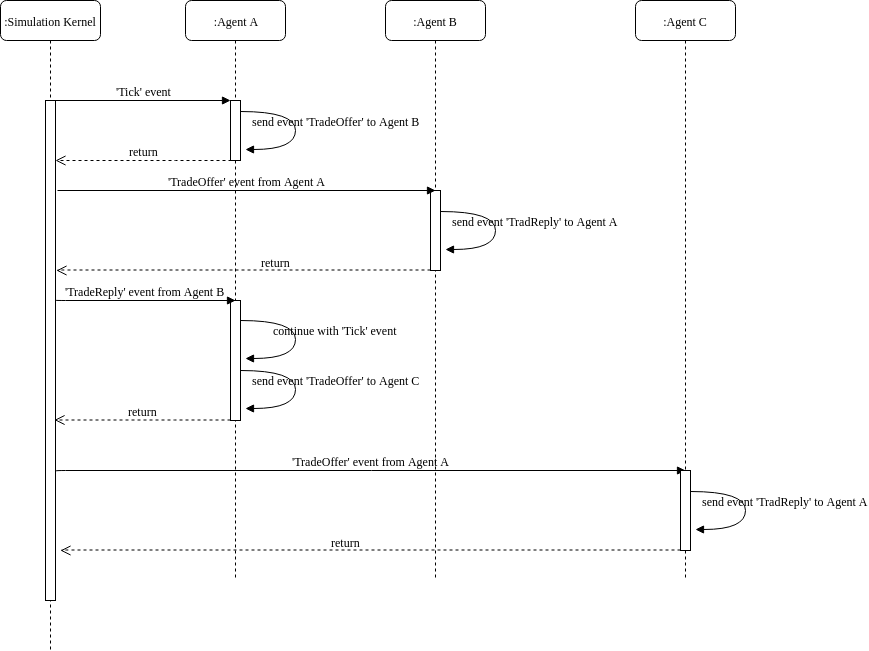
\includegraphics[width=1.0\textwidth, angle=0]{./fig/eventdriven/syncagentinteractions.png}
	\caption{Sequence diagram of synchronous agent interaction in the trading use-case. Upon the handling of the \textit{Tick} event, agent A looks for trading partners and finds agent B within its neighbourhood and sends a \textit{TradingOffer} message. Agent B replies to this message with \textit{TradeReply} and agent A continues with the trading algorithm by picking up where it has left the execution when sending the message to agent B. After agent A has finished the trading with agent B, it turns to agent C, where the same procedure follows.}
	\label{fig:syncagentinteractions}
\end{figure}

The way to implement this is to allow an agent to be able to change its internal event-handling state: to switch into different event-handlers, after having sent an event, to be able to react to the incoming reply in a specific way by encapsulating local state for the current synchronous interaction through closures and currying. Further, by making use of continuations the agent can pick up the processing of the \textit{Tick} event after the synchronous agent interaction has finished. Key to this is the function \textit{continueWithAfter} which we already shortly introduced through \textit{generalEventHandler}. This function takes an MSF which returns an output of type \textit{b} and an optional MSF. If this optional \textit{Maybe} MSF is \textit{Just} then the \textit{next} input is handled by this new MSF. In case no new MSF is returned (\textit{Nothing}), the MSF will stay the same. This is a more specialised version of the \textit{switch} combinator introduced in Chapter \ref{sec:back_frp} in the way that it doesn't need an additional function to produce the actual MSF continuation. Note that the semantics are different though: whereas \textit{switch} runs the new MSF immediately, \textit{continueWithAfter} only applies the new MSF in the \textit{next} step. The implementation of the function is as follows:

\begin{HaskellCode}
continueWithAfter :: Monad m => MSF m a (b, Maybe (MSF m a b)) -> MSF m a b
continueWithAfter msf = MSF (\a -> do
  ((b, msfCont), msf') <- unMSF msf a
  let msfNext = fromMaybe (continueWithAfter msf') msfCont
  return (b, msfNext))
\end{HaskellCode}

Finally, we can discuss the \textit{Tick} handling function. It returns a value of type \textit{Maybe (EventHandler g)} which if is \textit{Just} will result in to a change of the top-level event handler through \textit{continueWithAfter} as shown in \textit{generalEventHandler} above. Note the use of continuations in the case of \textit{agentMating, agentTrade} and  \textit{agentLoan}. All these functions return a \textit{Maybe (EventHandler g)} because all of them can potentially result in synchronous agent interactions which require to change the top-level event handler. The function \textit{agentDisease} is the last in the chain of agent behaviour, thus we are passing a default continuation which simply switches back into \textit{generalEventHandler} to finish the processing of a \textit{Tick} in an agent.

\begin{HaskellCode}
handleTick :: RandomGen g => DTime -> AgentLocalMonad g (Maybe (EventHandler g))
handleTick dt = do
  -- perform ageing of agent
  agentAgeing dt
  -- agent move, returns amount it of resources it harvested
  harvestAmount <- agentMove
  -- metabolise resources, depending on agents metabolism rate
  -- returns amount metabolised
  metabAmount <- agentMetabolism
  -- polute environment given harvest and metabolism amount
  agentPolute harvestAmount metabAmount

  -- check if agent has starved to death or died of age
  ifThenElseM
    (starvedToDeath `orM` dieOfAge)
    (do
      -- died of age or starved to deat: remove from simulation
      agentDies agentMsf
      return Nothing) 
    -- still alive, perform the remaining steps of the behaviour
    -- pass agentContAfterMating as continuation to pick up after mating
    -- synchronous conversations have finished
    (agentMating agentMsf agentContAfterMating)

-- after mating continue with cultural process and trading
agentContAfterMating :: RandomGen g => AgentLocalMonad g (Maybe (EventHandler g))
agentContAfterMating = do
    agentCultureProcess
    -- pass agentContAfterTrading as continuation to pick up after trading 
    -- synchronous conversations have finished
    agentTrade agentContAfterTrading 

-- after trading continue with lending and borrowing
agentContAfterTrading :: RandomGen g  => AgentLocalMonad g (Maybe (EventHandler g))
agentContAfterTrading = agentLoan agentContAfterLoan

-- after lending continue with diseases, which is the step in a Tick event
agentContAfterLoan :: RandomGen g => AgentLocalMonad g (Maybe (EventHandler g))
agentContAfterLoan = agentDisease defaultCont

-- safter diseases imply switch back into the general event handler
defaultCont :: RandomGen g => AgentLocalMonad g (Maybe (EventHandler g))
defaultCont = return (Just generalEventHandler)
\end{HaskellCode}

\subsubsection{Tagless final}
Although the indirect, continuation based approach to synchronous agent interactions as shown before works, it is quite cumbersome, fragile and it is easy to get something wrong. What would be more desirable is to have a truly synchronous approach, where the reply to an event happens directly as a result of the \textit{sendEventTo} function: when calling \textit{sendEventTo}, behind the scenes the receiving agent is executed and the result is returned directly to the caller, without any indirections. With the \textit{tagless final} approach as introduced in the event-driven SIR above, this becomes possible in an elegant and robust way. We have developed this concept for the event-driven SIR only. Still, it should be equally applicable for the Sugarscape but we leave that for further research.

We start by extending the API by defining a \textit{new} typeclass \textit{MonadAgentSync}:

\begin{HaskellCode}
class Monad m => MonadAgentSync e m | m -> e where
  sendSync :: e -> AgentId -> m (Maybe [e])
\end{HaskellCode}

The semantics behind the \textit{sendSync} method shall be that it allows to send an event of type \textit{e} to agent with id \textit{AgentId}. If the agent cannot be found it will return \textit{Nothing}, otherwise it will return \textit{Just} the list of events the receiving agent replies to the sending agent. 

The only place which has to be changed is the susceptible agent but due to the different semantics, parts of its behaviour needs to be rewritten. The receiving agents are left unchanged as at the moment a receiver has no means to distinguish between asynchronous and synchronous events and is not forced to reply to the sender in case of a synchronous event. It would be useful to have some mechanism that in case of a synchronous event, the receiver can only reply to the sender. We leave that issue for further research.

Handling an incoming \textit{Contact} from an \textit{Infected} is no longer necessary as it will not happen, because the interactions go directly through \textit{sendSync} and infected agents don't make contact pro-actively. Thus, the \textit{MakeContact} handler has to be changed to take into account that the infection can happen directly there:

\begin{HaskellCode}
handleEvent MakeContact = do
  ais        <- getAgentIds
  ai         <- getMyId
  isInfected <- makeContact beta ai ais
  if isInfected
    -- got infected, signal event to switch
    then return (Just ())
    else do
      -- not infected, re-schedule MakeContact
      scheduleMakeContact
      return Nothing
\end{HaskellCode}

The function \textit{makeContact} recursively \textit{makeContactWith} $\beta$ (contact rate) other agents. Whereas previously, sending a \textit{Contact} event to itself was not a problem, this is not allowed any more and must be prevented explicitly. The reason for that is discussed below in the implementation of the \textit{sendSync} method of the pure interpreter. Note that sending to itself counts against the $\beta$ contacts, as it would make no difference: receiving a \textit{Contact} from a \textit{Susceptible} has no effect on a susceptible agent anyway. If the case arises in a model that agents need to send events to themselves, it cannot happen through mechanisms like \textit{sendSync} but it has to go through asynchronous scheduling of events which decouples the sending from the receiving.

\begin{HaskellCode}
makeContact :: (MonadAgent SIREvent m, MonadAgentSync SIREvent m)
            => Int       -- ^ number of contacts to make
            -> AgentId   -- ^ sender agent id
            -> [AgentId] -- ^ all agent ids (including self)
            -> m Bool
makeContact 0 _ _ = return False
makeContact n ai ais = do
  receiver <- randomElem ais
  -- prevent sending to self
  if ai == receiver
    -- self counts against beta contacts
    then makeContact (n-1) ai ais
    else do
      -- make contact
      ret <- makeContactWith receiver
      if ret
        -- got infected, stop
        then return True
        -- not infected, continue
        else makeContact (n-1) ai ais
\end{HaskellCode}

Finally we can use \textit{sendSync} to directly send events to a receiving agent, which replies with a list of events to the sender. Note that we needed to add the new \textit{MonadAgentSync} typeclass to the overloaded function, to make the \textit{sendSync} method available.

\begin{HaskellCode}
makeContactWith :: (MonadAgent SIREvent m, MonadAgentSync SIREvent m) 
                => AgentId -> m Bool
makeContactWith receiver = do
  ai     <- getMyId
  -- DIRECT SYNCHRONOUS AGENT INTERACTION HAPPENS HERE
  retMay <- sendSync (Contact ai Susceptible) receiver
  case retMay of 
    -- receiver not found, no infection
    Nothing -> return False
    -- receiver found, replied with es events
    (Just es) -> do
      -- check if any event in replies is from Infected
      let fromInf = any (\ (Contact _ s) -> s == Infected) es
      if not fromInf
        -- none from Infected, no infection
        then return False
        -- at least one from Infected, might become infected
        else do
          r <- randomBool inf
          if r 
            -- got infected, become infected
            then do
              scheduleRecoveryM ild
              return True
            else return False
\end{HaskellCode}

The \textit{sendSync} method needs to be implemented in a new \textit{pure} interpreter, which follows exactly the same concept as before so we briefly discuss it conceptually. The method looks up the receiving agent, runs it with the given event of the sender and filters the replies to the sending agent. To do that, the method needs to have all agents available to actually execute them. This is achieved by keeping the agent mappings in the \textit{SimState}, introduced in the initial section on \textit{tagless final} of the event-driven SIR. They are managed using a \textit{State} Monad, thus can be read and written, which both is necessary as after a successful run of the receiving agent, its new MSF needs to be put back into the agent mappings.

Now it becomes clear why an agent cannot send an event with \textit{sendSync} to itself and why circular (agent A sendSync to agent B sendSync to agent C sendSync to agent A) \textit{sendSync} are also not allowed. The new MSF of an agent which was just run and updated in the \textit{SimState} will be overridden by the subsequent updates of runs which were initiated earlier. Fortunately, this can be conveniently checked within the \textit{sendSync} method and an error or exception can be generated which is better than silently ignoring it, resulting in unexpected behaviour. It is possible because the initiating agents id is always known and because it is easy to keep track of the agent ids currently engaged in a \textit{sendSync} by storing their ids in the \textit{SimState}, thus arriving at some kind of call stack management.

Although the very direct \textit{tagless final} agent interaction approach makes things under certain circumstances easier, it comes also with subtle drawbacks, thus it depends on the model semantics which approach to synchronous agent interactions should be chosen. Still we think that this approach is another demonstration of the usefulness of a \textit{tagless final} approach: we have shown how to extend the existing API with new operations without breaking the existing implementation. Also we think that we only scratched the surface with this approach of direct synchronous agent interactions but we leave a more in-depth exploration of it for further research.

%\section{Implementation Approaches}
5 Pages

This is now very programming-language specific

\begin{itemize}
	\item Mapping the strategies to 3 programming-languages: Java, Scala with Actors, Haskell
	\item Comparing the programming languages in regard of their suitability to implement each of these strategies
	\item Screen-shots of results of the same simulation-model with all the strategies
\end{itemize}

%\input{./tex/eventdriven/eventdrivenSIR.tex}

\section{Discussion}
Although there are similarities to the work of \cite{botta_time_2010} (the use of messages and the problem of when to advance time in models with arbitrary number synchronised agent-interactions), we approach our agents differently. First in our approach an agent is only a single MSF and thus can not be directly queried for its internal state / its id or outgoing messages, instead of taking a list of messages, our agents take a single event/message and can produce an arbitrary number of outgoing messages together with an observable state - note that this would allow to query the agent for its id and its state as well by simply sending a corresponding message to the agents MSF and requiring the agent to implement message handling for it. Also the state of our agents is \textit{completely} localised and there is no means of accessing the state from outside the agent, they are thus "fully encapsulated agents" \cite{botta_time_2010}. Note that the authors of \cite{botta_time_2010} define their agents with a polymorphic agent-state type \textit{s}, which implies that without knowledge of the specific type of \textit{s} there would be no way of accessing the state, rendering it in fact also fully encapsulated. The problem of advancing time in our approach is solved not exactly the same but conceptually it is the same: after sending a tick message to each agent (in random order), we process all agents until they are idle: there are no more enqueued messages / events in the queue.

our eventdriven approach makes heavy use of 2 state monads, thus one might ask what the benefits are, after all we seem to fall back into stateful, imperative style programming. we agree that our approach is just one way of implementing abs in fp but we think we have come a long way thus making our approach quite valuable even if there might be other approaches like shallow EDSLs. on the other hand even our stateful programming is highly restricted to only those 2 local datatypes which makes it much more manageable than unrestricted data mutation

quote carmack (\url{http://www.gamasutra.com/view/news/169296/Indepth_Functional_programming_in_C.php}): the main difficulty as a developer in software programming is to keep track of the states a program can be in and reason about them and their Validity

TODO: report LoC and compare it with other implementations we found on the internet